\documentclass[tikz]{standalone}
    \usepackage{tikz}
    \usetikzlibrary{positioning, graphs}
    \usetikzlibrary{graphs.standard}
    \usetikzlibrary{arrows.meta}
    \begin{document}
    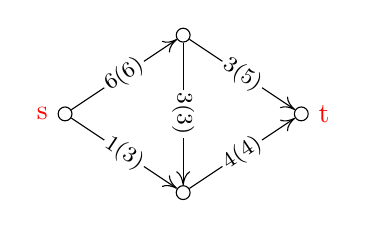
\begin{tikzpicture}
        [
            vertex/.style={draw,circle,inner sep = 0em, minimum size = 0.5em, fill=white},
            edgelabel/.style = {fill = white, inner sep = 0.1em, font=\footnotesize},
            nodelabel/.style = {color = red}
        ]
        \node[vertex, label = {[nodelabel]left : s}] (s) at (0, 0) {};
        \node[vertex] (a) at (1.5, 1) {};
        \node[vertex] (b) at (1.5, -1) {};
        \node[vertex, label = {[nodelabel]right : t}] (t) at (3, 0) {};
        
        \draw[-{>[length=5, width=5]}] (s) to node[edgelabel,sloped] {$6(6)$} (a);
        \draw[-{>[length=5, width=5]}] (s) to node[edgelabel,sloped] {$1(3)$} (b);
        \draw[-{>[length=5, width=5]}] (a) to node[edgelabel,sloped] {$3(3)$} (b);
        \draw[-{>[length=5, width=5]}] (a) to node[edgelabel,sloped] {$3(5)$} (t);
        \draw[-{>[length=5, width=5]}] (b) to node[edgelabel,sloped] {$4(4)$} (t);
    \end{tikzpicture}
    \end{document}